\chapter{Architektura}

Emulátor jakéhokoliv hardwarového systému je ve své podstatě velmi komplexní, 
proto je třeba správně rozvrhnout celkovou implementaci tohoto projektu. 
Zaprvé, je nezbytné myslet na udržitelnost kódu a schopnost jej bez větších problémů rozšiřovat. 
Za druhé, komplexita kódu by měla být rozdělena do jednotlivých jednotek.
Emulátor také potřebuje přístup k oknu a musí být schopen vykreslovat obsah grafické paměti na obrazovku.

\section{Nástroje}

Pro tyto účely a požadavky jsem zvolil \textit{C++} jako jazyk pro implementaci. 
\textit{Objektivně orientovaný} přístup k designu projektu a \textit{polymorfismus} tohoto jazyka jsou pro tento projekt ideální.

Pro přístup ke grafickému rozhraní jsem zvolil knihovnu \textit{SDL2}, což je univerzální 
nástroj pro otevírání oken v operačním systému a možnost kreslení do nich. \textit{SDL2} mimo jiné také umožňuje práci s obrázky a hudbou.

\section{Hardwarová komponenta}

\textit{PlayStation} ve svém hardwarovém designu připomíná velice obyčejný počítač, kterému byly odstraněny přebytěčné komponenty.
\textit{Sony}, na rozdíl od svých oponentů, vytvořilo tuto konzoli z relativně dobře dokumentovaných čipů již existujících počítačů. 
Samozřejmě \textit{PlayStation} obsahuje i patentované, na míru udělané, součástky, které se snaží ulehčit práci procesoru.

Tyto hardwarové čipy sdílejí velmi podobné rozhraní. 
To je dáno tím, že \textit{PlayStation} je nadesignován jako \textit{Memory-mapped I/O}.
To znamená, že sběrnice systému má uniformní paměťové rozložení, přičemž jednotlivé komponenty se mapují do specifických paměťových intervalů. 
Jednotlivé komponenty pak mohou do těchto intervalů zapisovat nebo číst a sběrnice pak rozdistribuuje tyto přístupy daným komponentám.
Díky tomuto faktu musí mít každá hardwarová komponenta následující schopnosti:

\begin{itemize}
    \item{\textit{Reset/Inicializace} komponenty}
    \item{\textit{Čtení} z komponenty}
    \item{\textit{Zápis} do komponenty}
    \item{Provedení \textit{jednotky práce} dané komponenty}
\end{itemize}

Pomocí dědičnosti a virtuálních metod v \textit{C++} můžeme specifikovat virtuální třídu, která bude sloužit jako základ pro všechny hlavní hardwarové komponenty.

\begin{figure}[hbt]
    \centering
    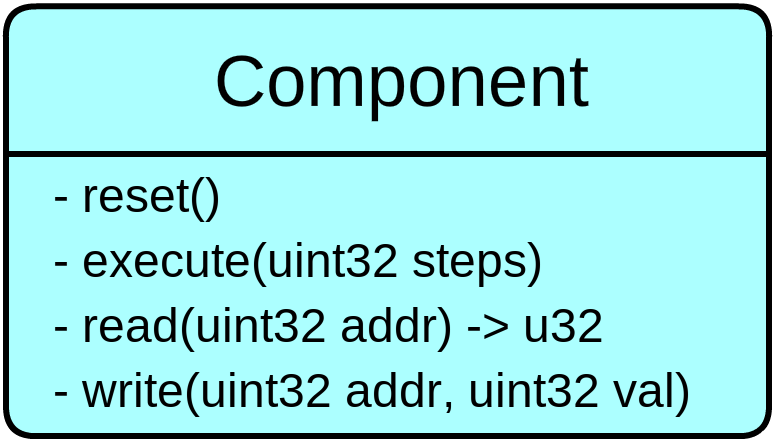
\includegraphics[width=0.4\textwidth]{obrazky-figures/component.png}
    \caption{Rozhraní, které každá hardwarová komponenta musí respektovat.}
    \label{component}
\end{figure}

\section{Návrh architektury}

\textit{PlayStation} se skládá z několika hlavních hardwarových komponent. Patří sem\cite{PSXSpec}:

\begin{itemize}
    \item Sběrnice
    \item Central Processing Unit \textbf{(CPU)}
    \item Graphics Processing Unit \textbf{(GPU)}
    \item Sound Processing Unit \textbf{(SPU)}
    \item 3 Časovače/Hodiny
    \item Ovladač přerušení
    \item Ovladač přímého přístupu do paměti \textbf{(DMA)}
    \item Dekodér makrobloku \textbf{(MDEC)}
    \item CD-ROM
\end{itemize}

Každá z těchto komponent je klíčová pro správné fungování emulátoru jako celku.
Detaily propojení komponent a schopností, s kým mohou komunikovat, jsou popsány v celkovém návrhu[\ref{psx-layout}].

\begin{figure}[hbt]
\centering
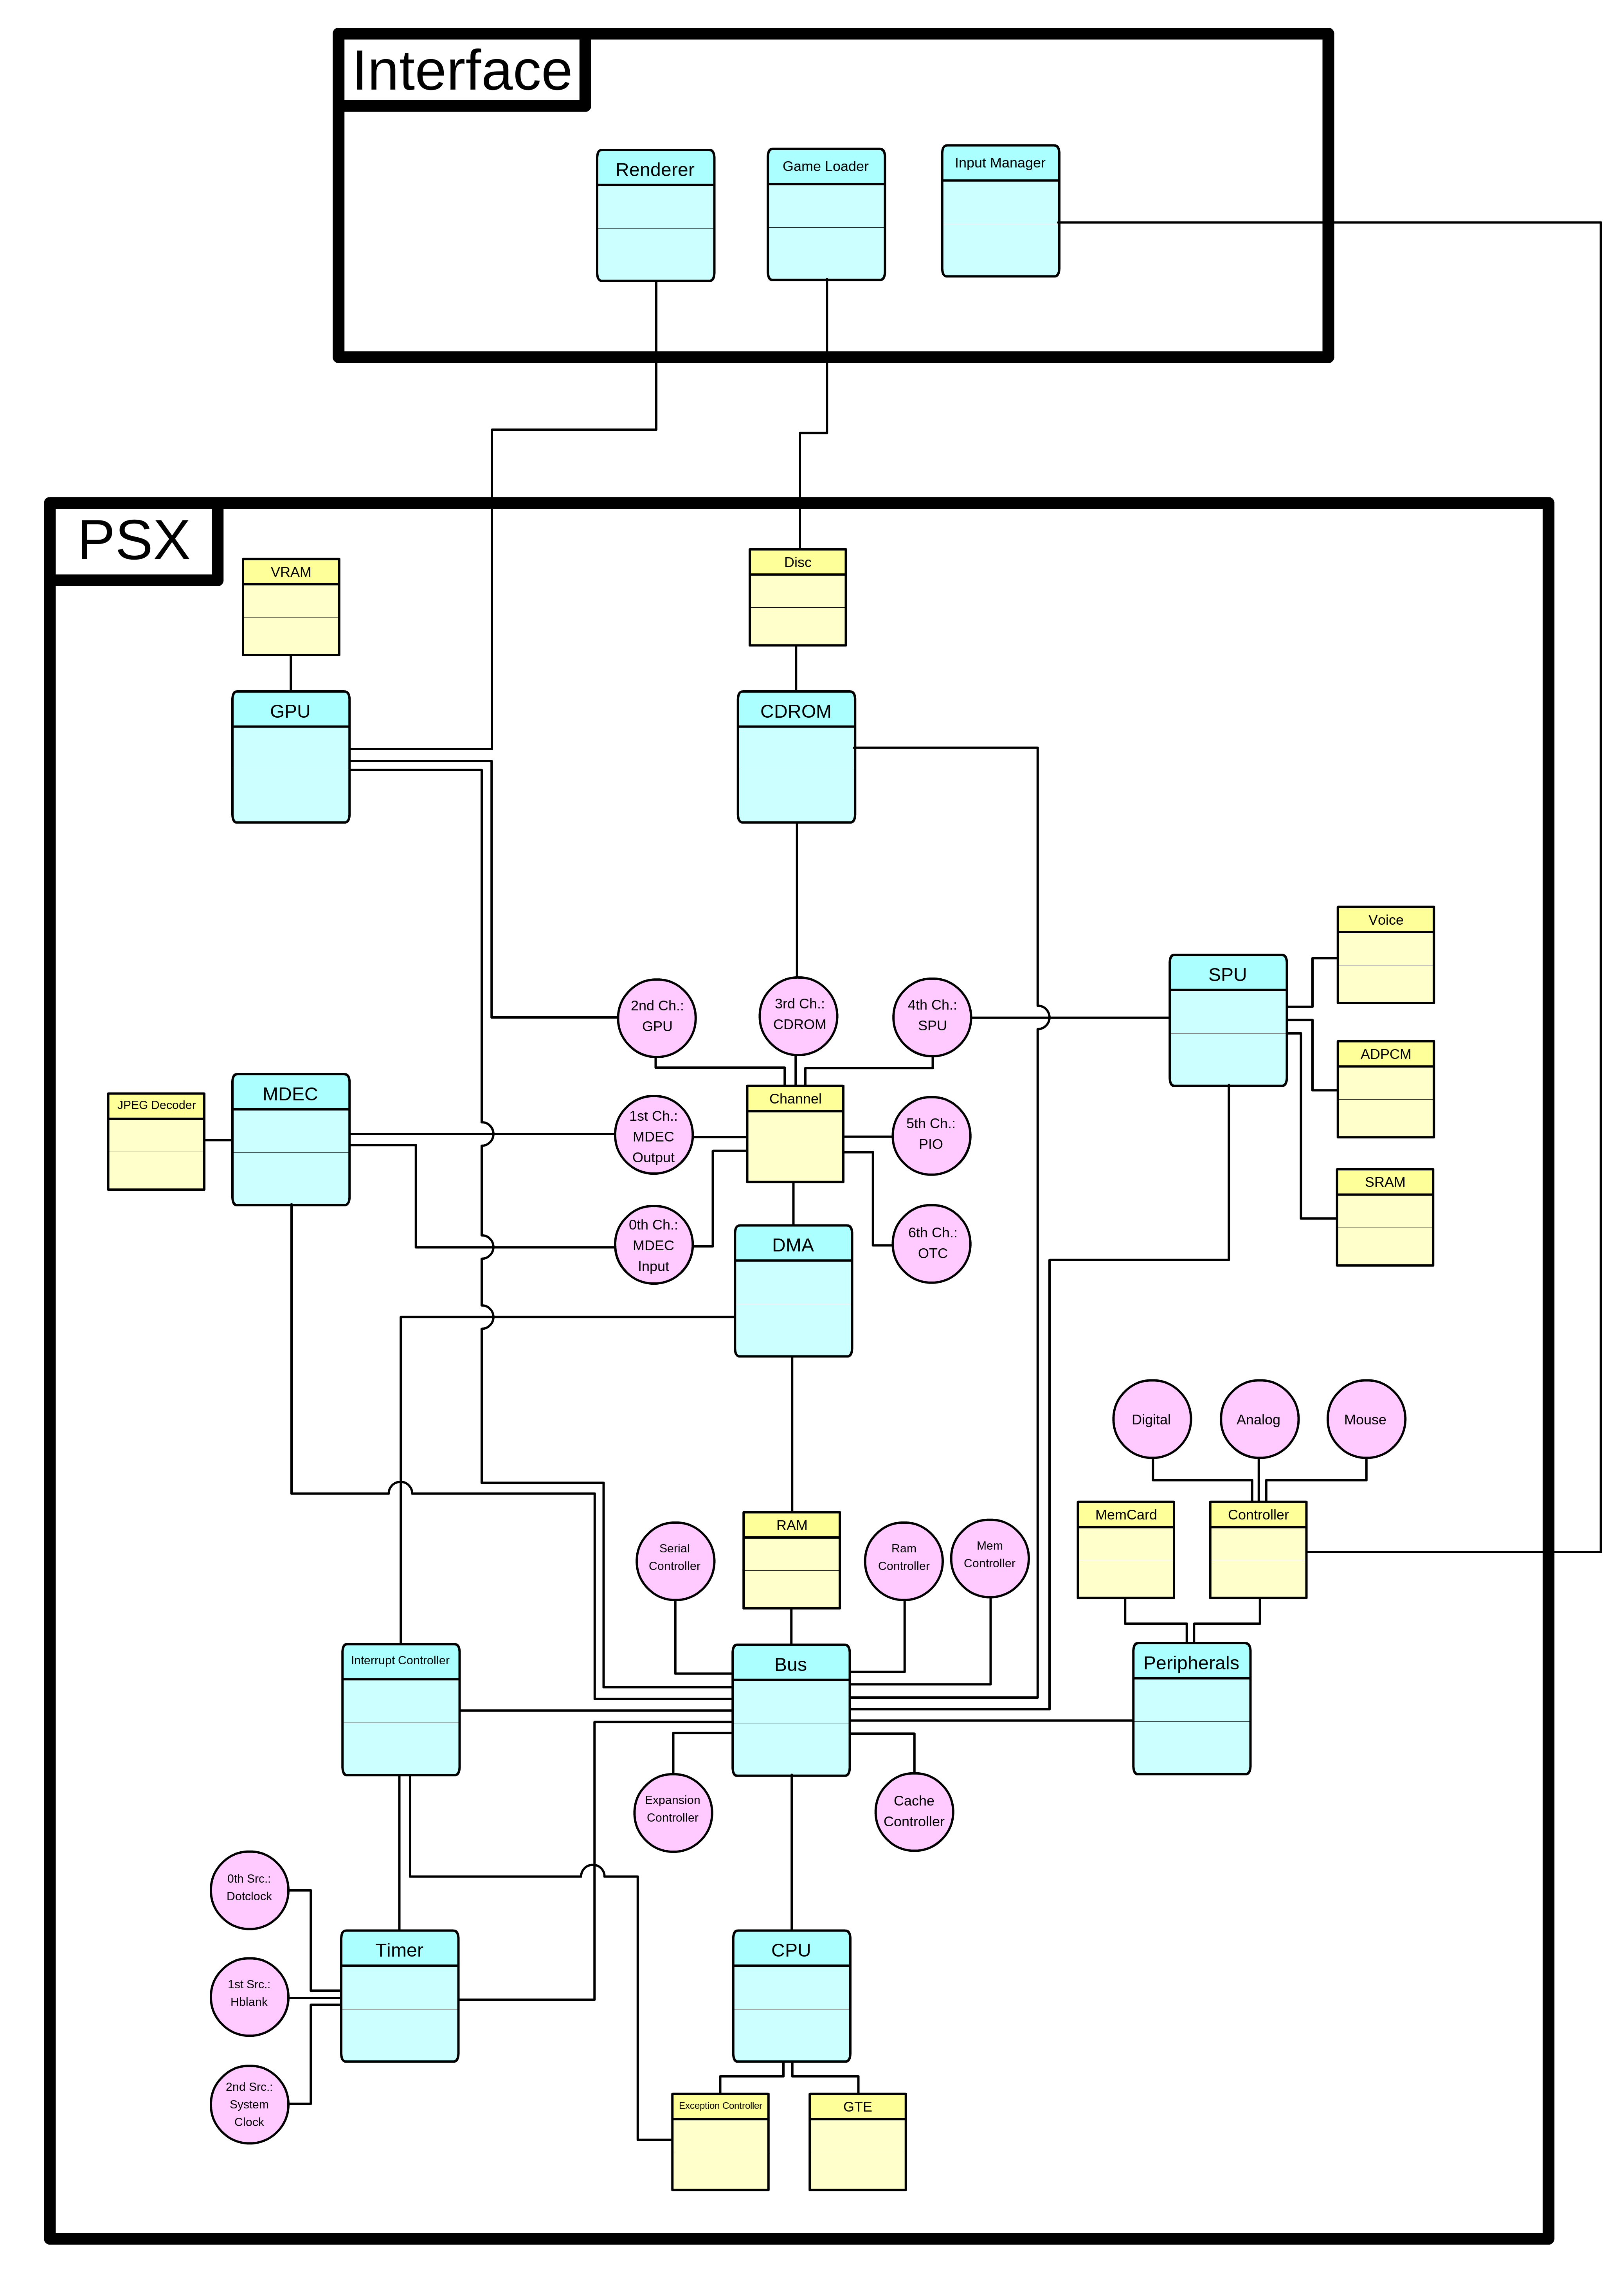
\includegraphics[width=1.0\textwidth]{obrazky-figures/psx-layout.png}
\caption{Kompletní návrh zapojení nejen hardwarových komponent emulátoru, ale i nadstavby nutné pro zpřístupnění stavu konzole.}
\label{psx-layout}
\end{figure}

V návrhu jsou také zohledněny podřadné komponenty, které nemohou fungovat samostatně.
To se týká například komponenty \textit{Geometry Transformation Engine (GTE)}, což je
ko-procesor specializující se na práci s lineární algebrou. Jelikož k této komponentě lze přistoupit
pouze skrze \textit{CPU} pomocí speciální instrukce, nelze tuto komponentu chápat jako samostatný celek.

Každá komponenta je následně propojena se sběrnicí kvůli \textit{Memory-mapped I/O}. Existují
však i přímá propojení bez sběrnice jako prostředníka. To je hlavně díky \textit{DMA} komponentě,
která zajišťuje rychlý přenos dat, aniž by se \textit{CPU} muselo starat o tento přenos. Další
přímá propojení jsou určena pro správu přerušení. Vzhledem k tomu, že přerušení může nastat skoro v
každé komponentě, je nutné toto přerušení přenášet do \textit{Ovladače vyjímek}, který následně
upraví stav \textit{CPU} a přerušení se zpracuje jako výjimka.